\section{Implementation Details}
\label{sec:implementation_details}

The pest detection system is implemented as a modern, web-based application that leverages a custom-trained YOLOv11 model for real-time agricultural pest identification. The core workflow, illustrated in Figure \ref{fig:architecture}, consists of several stages from data preparation to in-browser inference.

\begin{figure}[H]
    \centering
    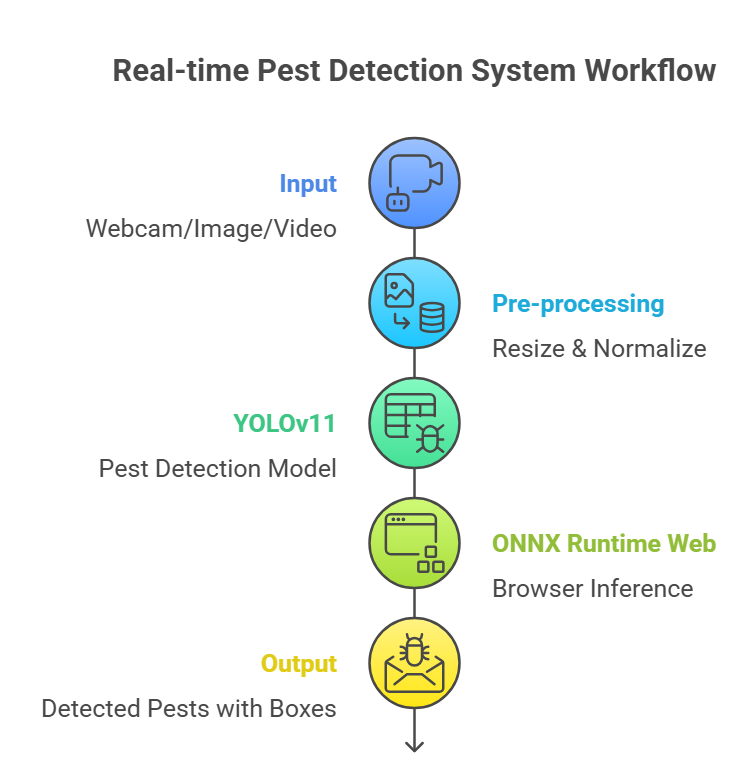
\includegraphics[width=0.8\columnwidth]{../images/architecture.png}
    \caption{System architecture diagram illustrating the workflow from data preparation to web-based inference.}
    \label{fig:architecture}
\end{figure}

\subsection{System Architecture and Workflow}

\subsubsection{Data Preparation and Preprocessing}
The system uses the "Insect Pest Detection in Agriculture using YOLO" dataset, which contains annotated images of various pest species. Preprocessing steps include resizing images to 640$\times$640 pixels, normalization, and extensive data augmentation (rotation, scaling, color jittering) to improve model generalization. The dataset is split into training, validation, and test sets (70\%, 20\%, 10\% respectively) [2].

\subsubsection{Model Training and Hyperparameters}
The YOLOv11 architecture was chosen for its balance of speed and accuracy. Training utilizes transfer learning with a pre-trained YOLOv11 nano model as the base. Key hyperparameters include 100 epochs, a batch size of 16, an initial learning rate of 0.01, and the AdamW optimizer. Techniques such as learning rate scheduling (cosine annealing), early stopping, and model checkpointing are employed to ensure optimal convergence and prevent overfitting [2, 5].

\subsubsection{Model Optimization and Deployment}
After training, the PyTorch model is exported to the ONNX format with dynamic input shapes and is then further optimized for web deployment using ONNX Runtime Web. The final model is converted to a `.ort` format, which significantly reduces model size and enables efficient inference in browser environments [2].

\subsubsection{Frontend User Interface}
The user interface is built with Next.js, React, TypeScript, and Tailwind CSS, ensuring a responsive and accessible design. The application supports three input modalities: live webcam feed, image upload, and video file processing. Detection results are visualized with bounding boxes and confidence scores overlaid on the input, and detailed JSON output is available for integration with external systems [1, 2].

\subsubsection{Inference Pipeline}
The ONNX Runtime Web engine runs the optimized model directly in the user's browser. The pipeline processes input frames, performs model inference, and applies post-processing (non-maximum suppression) to filter overlapping detections. Real-time performance metrics such as inference time and frames per second (FPS) are displayed to the user.

\subsection{Software Engineering and Best Practices}
The codebase is structured to maximize modularity, readability, and maintainability.

\subsubsection{Component-Based Design}
The frontend is organized into reusable React components, each responsible for a specific UI or logic function (e.g., input selection, result visualization, performance metrics display). This approach promotes separation of concerns and eases future enhancements.

\subsubsection{Type Safety and Documentation}
TypeScript is used throughout the frontend to enforce type safety and reduce runtime errors. Comprehensive inline documentation and clear naming conventions improve code readability and facilitate the onboarding of new contributors.

\subsubsection{Configuration Management}
Model parameters, inference settings, and UI options are managed via centralized configuration files, enabling easy adjustments and experimentation without requiring code changes.

\subsubsection{Testing and Error Handling}
The system includes robust error handling for file uploads, camera access, and inference failures. Unit and integration tests are implemented for critical components to ensure reliability.

\subsection{Performance and Optimization}
Several strategies were employed to ensure real-time performance and an efficient user experience.

\subsubsection{Iterative Processing for Real-Time Feedback}
For video and webcam streams, the system processes input frames in a continuous loop, applying the model to each frame and updating the UI in real time. This iterative approach ensures smooth and responsive detection, crucial for field deployment.

\subsubsection{Efficient Data Handling}
Image data is handled as multi-dimensional tensors, and detection results are stored in structured arrays for efficient rendering and downstream processing.

\subsubsection{Key Performance Optimizations}
The following optimizations were critical for achieving real-time performance on client-side devices:
\begin{itemize}
    \item \textbf{Model Optimization:} Conversion to ONNX and further optimization for WebAssembly reduces the model size to approximately 12MB and the memory footprint to under 200MB during inference, enabling real-time performance (16-22 FPS) on consumer hardware [2, 5].
    \item \textbf{Non-Maximum Suppression (NMS):} A greedy algorithm is used to efficiently filter overlapping bounding boxes, maximizing detection precision without significant computational overhead.
    \item \textbf{Asynchronous Operations and Lazy Loading:} The web application employs lazy loading for heavy components and asynchronous data processing to minimize UI blocking and improve the overall user experience.
\end{itemize}
